\documentclass[tikz,border=6pt]{standalone}
\usepackage{amsmath,amssymb}
\usepackage{xcolor}
\definecolor{accent}{HTML}{A13D2C}
\definecolor{accent2}{HTML}{2B5F6B}
\definecolor{muted}{HTML}{5A564F}
\definecolor{panel}{HTML}{F8F6F0}
\definecolor{linecol}{HTML}{D8D2C4}
\definecolor{astroblue}{HTML}{1B4F72}
\definecolor{sunyellow}{HTML}{E8A33D}
\definecolor{colthree}{RGB}{60,140,80}
\usetikzlibrary{calc,arrows.meta,plotmarks}
\IfFileExists{results/ch12/lane_emden_n3.dat}{\def\datadir{results/ch12/}}{\def\datadir{../results/ch12/}}
\usepackage[T1]{fontenc}\usepackage{newpxtext,newpxmath}  % same fonts as the notes
\begin{document}
% Lane-Emden solutions theta(xi) from code/ch12/01_lane_emden.py (cluster).
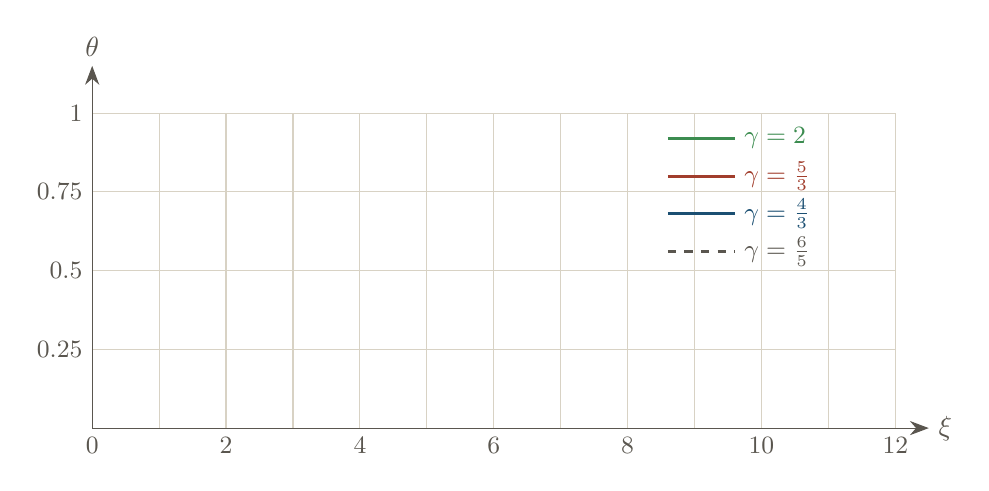
\begin{tikzpicture}[x=0.85cm,y=4cm, >={Stealth[length=2.4mm]}]
  \draw[linecol] (0,0) grid[xstep=1,ystep=0.25] (12,1);
  \draw[->, muted] (0,0) -- (12.5,0) node[right] {$\xi$};
  \draw[->, muted] (0,0) -- (0,1.15) node[above] {$\theta$};
  \foreach \x in {0,2,4,6,8,10,12} \node[below, muted] at (\x,0) {\small \x};
  \foreach \y in {0.25,0.5,0.75,1} \node[left, muted] at (0,\y) {\small \y};
  \draw[colthree, line width=1.1pt] plot file {\datadir lane_emden_n1.dat};
  \draw[accent, line width=1.1pt] plot file {\datadir lane_emden_n1.5.dat};
  \draw[astroblue, line width=1.1pt] plot file {\datadir lane_emden_n3.dat};
  \draw[muted, line width=1.1pt, dashed] plot file {\datadir lane_emden_n5.dat};
  \foreach \c/\lab/\y/\st in {colthree/{$\gamma=2$}/0.92/solid, accent/{$\gamma=\tfrac53$}/0.80/solid, astroblue/{$\gamma=\tfrac43$}/0.68/solid, muted/{$\gamma=\tfrac65$}/0.56/dashed} {
    \draw[\c, line width=1.1pt, \st] (8.6,\y) -- (9.6,\y); \node[\c, right] at (9.6,\y) {\small \lab};
  }
\end{tikzpicture}
\end{document}
